%!TEX root = main.tex
\chapter{Constraint Programming}

In this chapter we introduce the concepts of Constraint Programming, Constraint Satisfaction and \acf{CSP}. We also make a brief description of Constraint Programming history, known approaches and tools.

\section{Introduction}

This chapter introduces Constraint Programming, an alternative approach to programming which relies on a combination of techniques that deal with reasoning and computing~\cite{Apt2003}. Its definition actually comes from the field of Artificial Intelligence, and more specifically, arises from the concept of Constraint Satisfaction.

Constraint Satisfaction, in its most basic form, consists in finding a valid result for each set of problems. These sets of problems are modelled as \acp{CSP} which, in turn, specify sets of constraining relations between these problems. \acp{CSP} are defined in detail in Section~\ref{deeper}. 

\acp{CSP} have been tackled by the most various methods, from automata theory to ant algorithms and are a topic of interest in many fields of computer science~\cite{rossi2006handbook}.

\section{History of Constraint Programming}

Before understanding what Constraint Programming is, we need to understand that Constraint Satisfaction is the process of finding a solution to a set of constraints that impose conditions that the variables must satisfy~\cite{Apt2003}. A solution is found when a set of variables satisfies all constrains. These constraints and variables are described in detail in Section~\ref{deeper}.

Constraint Satisfaction originally appeared in the field of artificial intelligence in the early 1970s. During the 1980s and 1990s constraints started being embedded in programming languages, as they were being developed, and the term Constraint Programming started to take form. Examples of these programming languages are \textit{Prolog} and \textit{C++}~\cite{Apt2003}.

In the AI community interest in Constraint Satisfaction developed into two streams, the language stream and the algorithm stream. The first stream refers to the side of Constraint Satisfaction that deals with algebraic equations, constraint statements and declarative languages, while the second stream refers to the actual algorithms used to solve said constrains~\cite{rossi2006handbook}.

\section{Constraint Programming Concepts}
\label{deeper}

In this section we are going to introduce various important definitions related to \acp{CSP} as well how to model them and solve them.

\subsection{\acf{CSP}}

To solve a \ac{CSP} one must first model it. A \ac{CSP} is defined as a given set of $n$ variables to which each is assigned a well defined domain and a set of constraining relations and, in general, more than one representation of a problem as a \ac{CSP} exists. To solve a \ac{CSP} one must find all possible n-tuples, such that each $n$-tuple is an instantiation of the $n$ variables satisfying the relations~\cite{freuder1978synthesizing}. 

There are several definitions we have to delve into to better understand how \acp{CSP} work. We need to fully understand what a domain, a variable and a constraint are in this scope as well as how a \ac{CSP} is defined, modeled and solved. 

\subsection{Variable}

According to the field of elementary mathematics a variable is a symbol, usually an alphabetic character, and it represents a number, known as the value of the variable, which can be arbitrary, not fully specified or unknown~\cite{Menger1954}.

In more advanced mathematics, a variable is a symbol that denotes a mathematical object, which could be a number, a vector, a matrix or even a function~\cite{quine1960variables}. Similarly, in computer science a variable is a name (commonly an alphabetic character or a word) representing some value represented in computer memory.

\subsection{Domain}

According to Hans Hahn, from the field of mathematical analysis, an open set is connected if it cannot be expressed as the sum of two open sets. An open connected set is called a domain~\cite{hahn1921theorie}. In constraint programming, a domain is an open connected set of variables.

A bounded domain is a domain which is a bounded set, while an external domain is the interior of the complement of a bounded domain~\cite{miranda2012partial}. Carlo Miranda often used the term \textit{region} to identify an open connected set, while reserving the term \textit{domain} to identify an internally connected one.

\subsection{Constraint}

A constraint is a relation on the domains of a set of variables. It can be viewed as a requirement that states which combinations of values from the variable domains are allowed~\cite{Apt2003}.

During the modeling of a \ac{CSP} there can be two types of constraints. If the problem mandates that the constraints be satisfied, then the constraints are referred to has \textit{hard constraints}. However if in the problem it is preferred, but not required, that certain constraints be satisfied, then such non-mandatory constraints are referred to as \textit{soft constraints}.

\subsection{Modeling a \ac{CSP}}

\floatname{algorithm}{Listing}

\begin{algorithm}
    \caption{Modelling a \ac{CSP}}
    \label{modellingCSP}
    \begin{algorithmic}
        \State{}
        \State{$CSP = (V, D, C)$}
        \State{}
        \State{$V =\{V_1,V_2,\ldots,V_n\}$}
        \State{}
        \State{$D = \{D_1,D_2,\ldots,D_n\},\quad V_i \in D_i$}
        \State{}
        \State{$C = (C_1,C_2,\ldots,C_t), \quad C_j = (R_i,S_j)$}
        \State{}
    \end{algorithmic}
\end{algorithm}

Listing~\ref{modellingCSP} represents a classically modelled \ac{CSP}, according to Eugene C.Freuder and Alan K.Mackworth, as a triple $CSP = (V, D, C)$ where $V$ is an $n$-tuple of variables $V=(V_1,V_2,\ldots,V_n)$, D is a corresponding $n$-tuple of domains $D=(D_1,D_2,\ldots,D_n)$ such that $V_i \in D_i$, $C$ is a $t$-tuple of constraints $C=(C_1,C_2,\ldots,C_t)$. A constraint $C_j$ is a pair $(R_i,S_j)$ where $R_i$ is a subset of the Cartesian product of the domains of the variables in $S_i$~\cite{rossi2006handbook}.

\section{Approaches to Constraint Programming}

In Constraint Programming, we usually have a set of variables, which takes values from an initial domain, to which constraints are applied in order to reduce its domain, and thus reach a solution. Once a constraint is placed on the system it cannot violate another constraint previously applied. This way, we can express the requirements of the possible values of the variables~\cite{Pearson1997}.

\ac{CSP} are typically solved with the help of solvers. These solvers are essentially search algorithms, usually based on backtracking techniques\cite{Knuth1997}, constraint propagation \cite{Lecoutre2010} or local search \cite{Dechter2003}. 

\subsection{Backtracking}

Backtracking search is a basic control structure in computer science and finds a particular application in artificial intelligence. As the search is in general exponential in the number of variables, it is particularly helpful to have some means of obtaining bounds on the effort required for individual problems or classes of problems~\cite{freuder1985sufficient}. 

Backtracking searches incrementally and finds possible candidates to solve the problem. At the same time, it removes the candidates that can not be used as a valid solution to the problem~\cite{Knuth1997}. One of the most used examples for this type of search method is the n-queens puzzle, where a set of $n$ queens should be organized, in a $n \times n$ chess board, in such a way that none of the queens can attack each other. Any partial solution that contains two queens that can attack each other is abandoned immediately. The modelling can be seen in Section~\ref{nqueens}.

\subsection{Constraint Propagation}

Constraint propagation is the basic operation in Constraint Programming. It is well-recognized that its extensive use is necessary when efficiently solving hard \acp{CSP}. Almost all constraint solvers use it as a basic step~\cite{bessiere2001refining}.

Constraint propagation uses semantics of constraints to identify and discard incompatible combinations of values. Such combinations, which are instantiations that cannot be part of any solution, are called \textit{nogoods}. A typical way to propagate constraints is by reducing the domains of variables or the relations of constraints, resulting in a simpler search space to work on because all the \textit{nogoods} are now identified and can be used to avoid exploration of useless parts in the search space. 

Constraint propagation cannot, however, be used on it's own because it is only used to simplify a problem while maintaining its semantics so as to make it easier to solve. Some other algorithm must be then used to find the solutions or even optimal solutions~\cite{Lecoutre2010}.

\subsection{Local Search}

Local search methods date back over thirty years ago. Applied to difficult combinatorial optimization problems, this heuristic approach yields high-quality solutions by iteratively considering small modifications of a good solution in the hope of finding a better one~\cite{lin1965computer}.

Local search methods generally involve going from one solution to another repeatedly, achievable only through a local move, where valid moves can vary from problem to problem. The set of all solutions, reachable from the initial solution $S$ through a local move is called the neighborhood of $S$. The set of all probable solutions in the neighborhood of $S$ is called its probable neighborhood. To find the optimal solution, a strategy called \textit{iterative improvement} moves, on each iteration, to the best probable neighbor (the least costly) until it can't improve on the current solution~\cite{jussien2002local}.

Of course, this strategy has a very obvious drawback, and because of this several ways of alleviating the drawback have been proposed, such as multi-start iterative improvements and genetic local search~\cite{holland1992adaptation}. Both of these apply iterative improvements. The first one builds a pool of solutions and returns the best one while the second one discards the least-promising solutions and repeats the process until some stopping criteria is satisfied~\cite{jussien2002local}.

\section{Known Constraint Programming Solvers}

To reach a solution to a \ac{CSP} a Solver is needed. A various number of Constraint Programming Solvers exist, we present some of the most used ones in this section. Special attention should be placed on Choco, because this is the tool we chose to use in our constraint solving problem.

\subsection{Choco}

Choco is an open source and free access library dedicated to Constraint Programming. It is written in Java and supports several types of variables, including Integers, Booleans, Sets and Reals. It also supports several types of constraints such as AllDifferent and Count, configurable search algorithms and conflict explaining. It aims at describing real combinatorial problems in the form of \acp{CSP} and solving them with Constraint Programming techniques. Choco is used for teaching, researching and real life-applications~\cite{aboutChoco}~\cite{chocoSolver}.

The first version of Choco was developed in the early 2000s. A few years later, Choco 2 was developed and declared a success in the academic and industrial world. Since then, Choco has been completely re-written and in 2012 the third version of Choco was launched. The current version comes with a simpler API and is called Choco~\cite{historyChoco}~\cite{chocoSolver}.

Choco is among the fastest \ac{CSP} solvers on the market. In 2013 and 2014, Choco was awarded two silver medals and three bronze medals at the MiniZinc Challenge that is the world-wide competition of Constraint Programming solvers~\cite{aboutChoco}~\cite{chocoSolver}.

\subsection{Gecode}

Gecode is a free access, open source, portable, accessible and efficient programming environment used to develop systems and applications based on Constraints. Gecode, much like Choco, supports various types of variables and constraints, among them are Integers, Float and Sets. These variables are used to model problems that are then solved with the help of constraint propagators and search algorithms~\cite{schulte2010modeling}~\cite{gecode}.

Gecode is one of the fastest \ac{CSP} solvers, it won all gold medals in all categories in the MiniZinc Challenges from 2008 to 2012~\cite{gecode}.

\subsection{Google OR-Tools}

Although Choco and Gecode are two of the most widely used libraries, there are also other new tools, such as the Google OR-Tools~\cite{ORTools}. Google Optimization Tools or OR-Tools is an interface that puts together several linear programming solver and that counts on the use of several types of algorithms such as search algorithms and graph algorithms. What this library has that is so noteworthy is the fact that it doesn't let itself be bound by one language. Although implemented in C++, it can be used in other languages like Python, C\# or Java~\cite{ORTools}.

\section{Classic Constraint Problems}

In this section we present some classic constraint problems along with their modelling.

\subsection{$N$ Queens}
\label{nqueens}

The $n$ queens problem is, fundamentally, placing $n$ chess queens on an $n \times n$ chessboard so that no two queens attack each other~\cite{rivin1994n}. A feasible solution for this problem would be one in which no two queens share the same row, column or diagonal~\cite{hoffman1969constructions}.

The original $n$ queens problem was introduced by Gauss, in 1850, with an $n$ value of 8~\cite{hoffman1969constructions} and a total of 72 solutions, but soon after 92 solutions where theorized and in 1874 proved~\cite{rivin1994n}. For a board like this, one of the possible solutions can be seen in figure~\ref{fig:queens}.

\begin{figure}[hb]
    \centering
    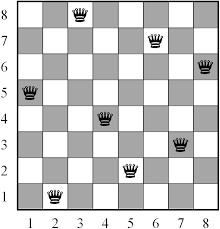
\includegraphics[width=50mm]{queens.png}
    \caption{Possible solution to the 8 queens problem}
    \label{fig:queens}
\end{figure}

By treating the chessboard as an $n \times n$ matrix of square elements, any square can be identified by an ordered pair $(i, j)$ where $i$ and $j$ are row and column numbers respectively. A major diagonal of the matrix can be identified by $m-j+i = CONSTANT$ where the $CONSTANT$ is the number of the diagonal. We can further define a minor diagonal with $i+j-1 = CONSTANT$ where $CONSTANT$ is the number of the diagonal~\cite{hoffman1969constructions}. 
The following constraints must always be applied to the $n$ queens problem:
\begin{itemize}
    \item a) The row numbers are unique.
    \item b) The column numbers are unique.
    \item c) The major diagonal numbers are unique.
    \item d) The minor diagonal numbers are unique.
\end{itemize}

\subsection{Sudoku}

According to J. Scott Provan, Sudoku is a logic-based, combinatorial number placement puzzle that can be defined by a set $S$ of $n$ grid squares that each have a possible placement of numbers from a set $P=\{1,\ldots,m\}$, a collection of blocks $\beta$ where each block consists of a set of exactly $m$ squares and an initial assignment of numbers in some grid squares. The goal is to assign numbers from $P$ to each of the remaining squares of $S$ in a way that each block $\beta$ has a complete set $P$ of non repeated numbers~\cite{provan2009sudoku}.

The typical Sudoku puzzle has a $m \times m$ configuration, and the usual value of $m$ is 9, which brings the value of $n$ to a total of 81 grid squares. On top of having to comply with the constraint of non repeating numbers in a block, the typical Sudoku puzzle also can not have repeating numbers in each row and column.

One requirement is that every Sudoku puzzle must have exactly one solution~\cite{provan2009sudoku}. An example of a standard Sudoku puzzle can be seen in figure~\ref{fig:sudoku} along with it's solution.

\begin{figure}[hb]
    \centering
    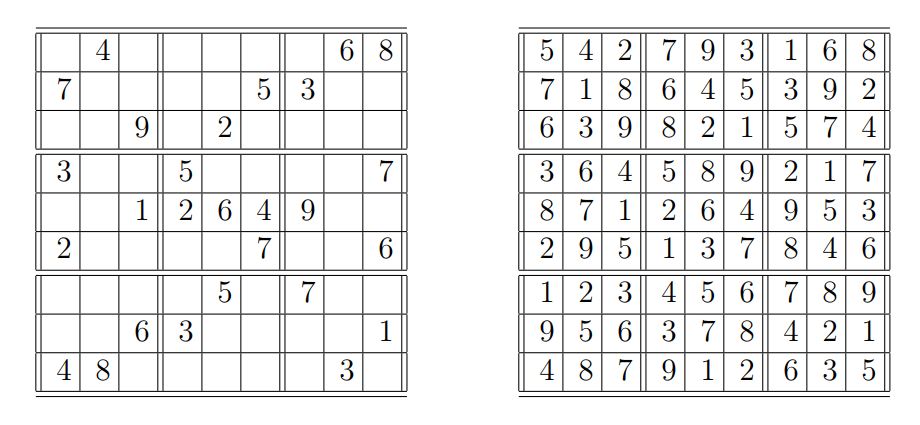
\includegraphics[width=120mm]{sudoku.png}
    \caption{Sudoku puzzle with respective solution}
    \label{fig:sudoku}
\end{figure}